\documentclass[a4paper, 12pt]{letter}
\usepackage[utf8]{inputenc}
\usepackage[scaled]{helvet}
\renewcommand\familydefault{\sfdefault}
\usepackage[T1]{fontenc}
\usepackage[francais]{babel}
\usepackage[left=2.5cm,top=6cm,right=2.5cm,bottom=2.5cm]{geometry}
\usepackage{graphicx}


\begin{document}
\pagenumbering{gobble} %no page number


\hbox to \textwidth{\hfill
	\vbox{
		\hbox{Monsieur}
		\hbox{Nelson José Bandarra Da cruz}
		\hbox{Rue Gilbert 44}
		\hbox{1217 Meyrin}
		\bigbreak
		\bigbreak
		\bigbreak
		\hbox{Veyrier, le 5 août 2016 / sl}
	}
}

\bigbreak



\begin{flushleft}
\textbf{Réponse négative}
\line(1,0){455}
\end{flushleft}
\bigbreak
Monsieur,

Nous accusons réception de votre candidature du 28 juillet 2016 qui a retenu toute notre attention et nous vous remercions de l’intérêt manifesté pour l’EMS Les Châtaigniers.

Malheureusement, sans que cela ne remette en cause la qualité de votre candidature, nous sommes au regret de vous informer que nous ne pouvons lui apporter une suite favorable, car nous n’avons à ce jour aucun poste vacant.

Dès lors, nous vous encourageons à déposer votre candidature en ligne sur le site de l’AGEMS (Association Genevoise des établissements médico-sociaux).

Nous vous souhaitons de trouver rapidement une opportunité conforme à vos aspirations et vous adressons, Monsieur, nos sincères salutations.

\bigbreak
\bigbreak
\bigbreak
\bigbreak

\hbox to \textwidth{\hfill
	\vbox{
		\hbox{EMS Les Châtaigniers}
	}
}

\begin{flushright}
		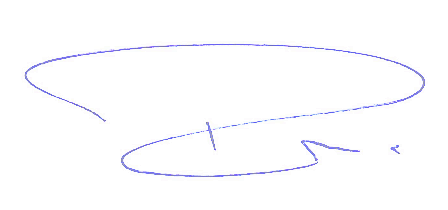
\includegraphics{sign.png}
		\end{flushright}

\hbox to \textwidth{\hfill
	\vbox{
		\hbox{Samuel Moix, Directeur adjoint}
	}
}

\bigbreak
\bigbreak

Annexe : votre dossier

\end{document}
